\documentclass{beamer}
\usepackage{xeCJK}
\usetheme[red,colorblocks]{Verona}
\usepackage{siunitx}
\usepackage{physics}
\usepackage{tikz,tikzpagenodes}
\usetikzlibrary{fadings}

%设置字体
\def\mathfamilydefault{\rmdefault}

%大纲格式:
%\numexpr\inserttocsectionnumber-1\relax
%只是为了在不知道 \inserttocsectionnumber 的计数器的情况下(Beamer 的说明文档里也没有,直接改 section 的计数器也没用,非常欢迎大家谁知道应该怎么改这个计数器了后告知我!)插入 5.0 节的一个技巧(
\setbeamertemplate{section in toc}{\hspace*{1em}5.\the\numexpr\inserttocsectionnumber-1\relax~\inserttocsection\par}
\setbeamertemplate{subsection in toc}{\hspace*{2em}5.\the\numexpr\inserttocsectionnumber-1\relax.\inserttocsubsectionnumber.~\inserttocsubsection\par}
\setbeamerfont{subsection in toc}{size=\normalsize}
\setbeamerfont{section in toc}{size=\large}
\AtBeginSection
{
	\begin{frame}
	    \frametitle{Content}
		\textbf{\tableofcontents[currentsection]}
	\end{frame}
}

%在右上角添加 logo
\addtobeamertemplate{frametitle}{}{%
\begin{tikzpicture}[remember picture,overlay]
\node[anchor=north east,yshift=2pt] at (current page.north east) {
\includegraphics[height=0.85cm]{标志与中英文校名组合规范_左右.png}};
\end{tikzpicture}}

%设置浅色渐变
\setbeamercovered{transparent}

\title{The LS-coupling scheme}
\subtitle{Atomic Physics Chapter 5}
\author{李昊润}
\institute[PKU]{School of Physics, Peking University}
\date{July 2024}

\begin{document}

%标题页
\begin{frame}[plain]
    \titlepage
    \begin{tikzpicture}[remember picture, overlay]
        \node[above left] at ([shift={(-0.5cm,0.5cm)}]current page.south east) {
\includegraphics[width=4cm]{标志_红色.png}};
    \end{tikzpicture}
\end{frame}

%正文
\section{Hamiltonian\&The LS-coupling scheme without fine structure}

\begin{frame}{Hamiltonian}
\uncover<1->{
    \begin{block}{The central-field approximation}
        \begin{equation*}
            \begin{aligned}
                V_{\mathrm{CF}}\left(r\right)&=-\frac{Ze^2/4\pi\epsilon_0}r+S(r),\\
                H_{\mathrm{CF}}&=\sum_{i=1}^N\left\{-\frac{\hbar^2}{2m}\nabla_i^2+V_{\mathrm{CF}}\left(r_i\right)\right\}.
            \end{aligned}
        \end{equation*}
    \end{block}}
\uncover<2->{
    The residual electrostatic interaction:
    \begin{equation*}
        H_{\mathrm{re}}=\sum_{i=1}^N\left\{\sum_{j>i}^N\frac{e^2/4\pi\epsilon_0}{r_{ij}}-S(r_i)\right\},
    \end{equation*}}
\uncover<3->{
    Hamiltonian:
    \begin{equation*}
        H=H_{\mathrm{CF}}+H_{\mathrm{re}}+H_{\mathrm{s-o}}.
    \end{equation*}}
\end{frame}

\begin{frame}{Hamiltonian}
\uncover<1->{
    It is generally very difficult to calculate the eigenvalues of the above Hamiltonian, so two extremes are usually discussed.}
    \begin{enumerate}
        \item<2-> LS-coupling scheme:
        \begin{equation*}
            H_{\mathrm{s-o}}\ll H_{\mathrm{re}}: H_{\mathrm{s-o}}{\to}\text{perturbation}, \text{basic quantum numbers}: LSJM_J,
        \end{equation*}
        \item<3-> jj-coupling scheme:
        \begin{equation*}
            H_{\mathrm{s-o}}\gg H_{\mathrm{re}}: H_{\mathrm{re}}{\to}\text{perturbation}, \text{basic quantum numbers}: n_il_ij_iJM_J.
        \end{equation*}
    \end{enumerate}
\end{frame}

\begin{frame}{LS-coupling scheme without fine structure}
\uncover<1->{
    \begin{block}{Hamiltonian}
        \begin{equation*}
            \begin{aligned}
                H&=\sum_{i=1}^N\left[-\frac{\hbar^2}{2m}\nabla_i^2+V_{\mathrm{CF}}\left(r_i\right)+\left\{\sum_{j>i}^N\frac{e^2/4\pi\epsilon_0}{r_{ij}}-S(r_i)\right\}\right],\\
                H&=H_{\mathrm{CF}}+H_{\mathrm{re}}.
            \end{aligned}
        \end{equation*}
    \end{block}}
\uncover<2->{
    Consider
    \begin{equation*}
        \boldsymbol{L}=\sum_i\boldsymbol{l}_i,\quad\boldsymbol{S}=\sum_i\boldsymbol{s}_i,\quad\boldsymbol{J}=\boldsymbol{L}+\boldsymbol{S}.
    \end{equation*}}
\uncover<3->{
    No external torque:
    \begin{equation*}
        \left[\boldsymbol{L}^2,H_\mathrm{re}\right]=0\quad\mathrm{~and~}\quad\left[{L}_z,H_\mathrm{re}\right]=0\mathrm.
    \end{equation*}}
\uncover<4->{
    $H_\mathrm{re}$ doesn't depend on spin:
    \begin{equation*}
        \left[\boldsymbol{S}^2,H_\mathrm{re}\right]=0\quad\mathrm{~and~}\quad\left[{S}_z,H_\mathrm{re}\right]=0.
    \end{equation*}}
\end{frame}

\begin{frame}{LS-coupling scheme without fine structure}
\uncover<1->{
    Therefore,
    \begin{equation*}
        \begin{aligned}
            \text{good quantum numbers}&: L,M_L,S,M_S,\\
            \text{eigenstates of} H_\mathrm{re}&: \ket{LM_LSM_S}.
        \end{aligned}
    \end{equation*}}
\uncover<2->{
    Label: 
    \begin{equation*}
        \textbf{terms}: {}^{2S+1}L_J.
    \end{equation*}}
\uncover<3->{
    \begin{block}{e.g. 3p4p in silicon}
        \begin{equation*}
            \begin{aligned}
                l_{1}&=1,& l_{2}&=1&\Rightarrow\quad L&=0,1\mathrm{~or~}2,\\
                s_{1}&=\frac{1}{2},& s_{2}&=\frac{1}{2}&\Rightarrow\quad S&=0\mathrm{~or~}1,\\
            \end{aligned}
        \end{equation*}
        \begin{equation*}
            \text{terms (without J) }:\quad {}^{2S+1}L={}^{1}\mathrm{S,}^{1}\mathrm{P,}^{1}\mathrm{D,}^{3}\mathrm{S,}^{3}\mathrm{P,}^{3}\mathrm{D}.
        \end{equation*}
    \end{block}}
\end{frame}

\begin{frame}{Energy levels}
\uncover<1->{
    Isotropy: degeneracy with respect to $M_L$ and $M_S$.}
    \begin{columns}
    \hspace*{1em}
    \column{0.51\textwidth}<2->
        \begin{figure}
            \centering
            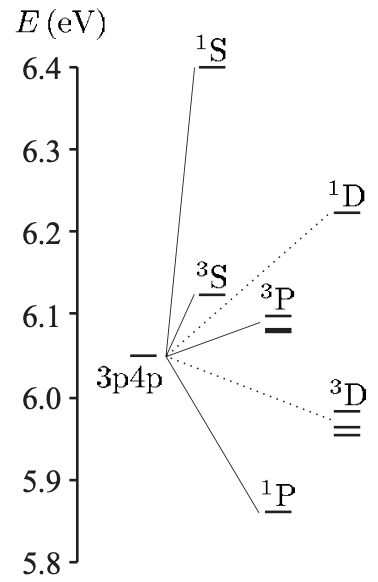
\includegraphics[scale=0.32]{fig/fig 5.1.png}
            \caption{3p4p in silicon}
        \end{figure}
        \begin{block}{Degenerate states}
            \begin{equation*}
                (2l_1+1)(2l_2+1)(2s_1+1)(2s_2+1)=36.
            \end{equation*}
        \end{block}
    \column{0.5\textwidth}<3->
        \begin{figure}
            \centering
            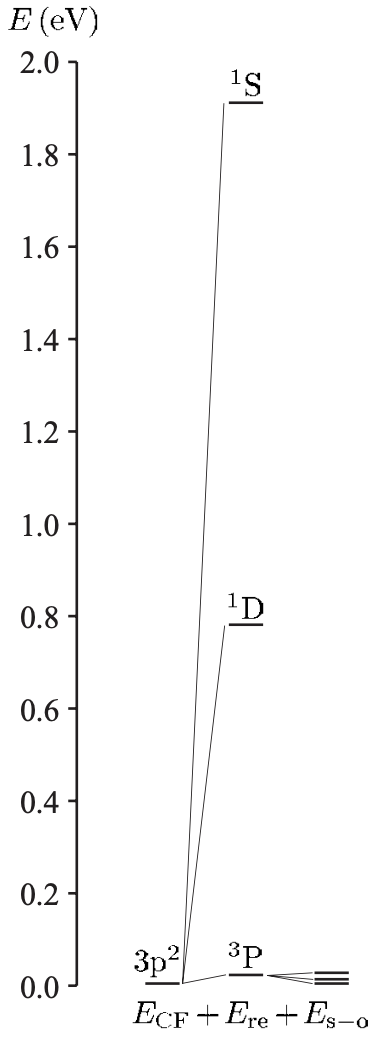
\includegraphics[scale=0.32]{fig/fig 5.2.png}
            \caption{$\mathrm{3p}^2$ in silicon}
        \end{figure}
    \end{columns}
\end{frame}
\section{Fine structure in the LS-coupling scheme}

\begin{frame}{Fine structure in the LS-coupling scheme}
\uncover<1->{
    \begin{block}{Spin orbit coupling of electrons}
        Approximate calculations of relativistic quantum mechanics at low speeds: 
        \begin{equation*}
            U_{sl}=\frac{1}{2\mu^{2}c^{2}}\frac{1}{r}\frac{\mathrm{d}U}{\mathrm{d}r}\boldsymbol{s}\cdot\boldsymbol{l}=\xi(r)\boldsymbol{s}\cdot\boldsymbol{l}.
        \end{equation*}
    \end{block}}
\uncover<2->{
    The Hamiltonian:
    \begin{equation*}
        \begin{aligned}
            H_{\mathrm{s-o}}&=\sum_{i}\beta_i\boldsymbol{s}_i\cdot\boldsymbol{l}_i=\beta_{LS}\boldsymbol{S}\cdot\boldsymbol{L}.\\
            H&=H_{\mathrm{CF}}+H_{\mathrm{re}}+H_{\mathrm{s-o}}.
        \end{aligned}
    \end{equation*}}
\uncover<3->{
    the total electronic angular momentum: $\boldsymbol{J}=\boldsymbol{L}+\boldsymbol{S}$.
    \begin{gather*}
        \because\quad\boldsymbol{L}\cdot\boldsymbol{S}=\frac{\left(\boldsymbol{J}\cdot\boldsymbol{J}-\boldsymbol{L}\cdot\boldsymbol{L}-\boldsymbol{S}\cdot\boldsymbol{S}\right)}{2},\\
        \therefore\quad\left[\boldsymbol{J}^2,H\right]=0\quad\mathrm{~and~}\quad\left[{J}_z,H\right]=0.
    \end{gather*}
    }
\end{frame}

\begin{frame}{Fine structure in the LS-coupling scheme}
\uncover<1->{
    Therefore, $L_z, S_z$ are no longer conserved.
    \begin{equation*}
        \begin{aligned}
            \text{good quantum numbers}&: L,S,J,M_J,\\
            \text{eigenstates of} H&: \ket{LSJM_J}.
        \end{aligned}
    \end{equation*}}
\uncover<2->{
    The energy shift: (degeneracy with respect to $M_J$)
    \begin{equation*}
        \begin{aligned}
            E_{{\mathrm{s-o}}}&=\beta_{LS}\left\langle\boldsymbol{S}\cdot\boldsymbol{L}\right\rangle\\
            &=\frac{\beta_{LS}}{2}\left\{J\left(J+1\right)-L\left(L+1\right)-S\left(S+1\right)\right\}.
        \end{aligned}
    \end{equation*}}
\uncover<3->{
    \begin{block}{Lande interval rule}
        The energy interval between adjacent $J$ levels: 
        \begin{equation*}
            \Delta E_{{\mathrm{FS}}}=E_{J}-E_{J-1}=\beta_{LS}J\propto J.
        \end{equation*}
    \end{block}
    }
\end{frame}

\begin{frame}{Example: pp electronic configuration}
\only<1>{
    \begin{block}{$n\mathrm{p}n'\mathrm{p}\ (n\neq n')$}<1>
        \centering
        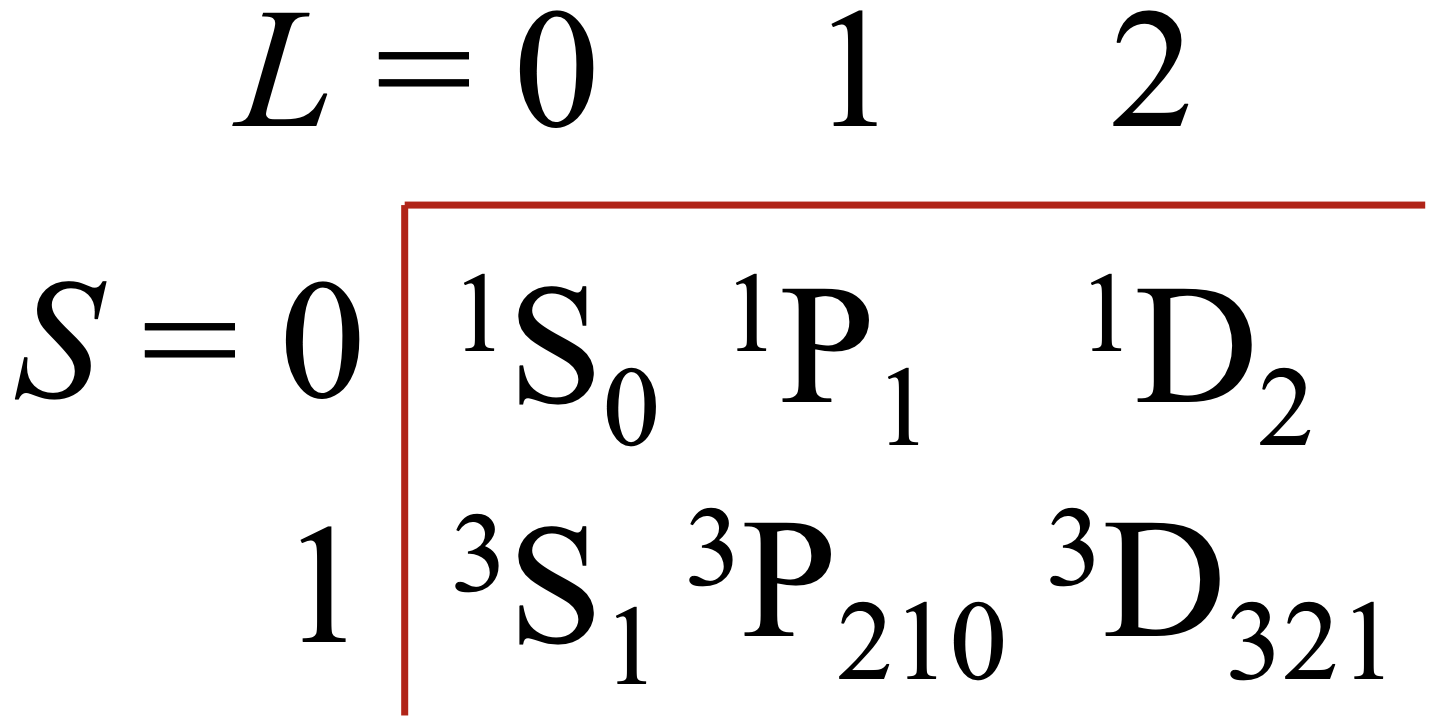
\includegraphics[scale=0.2]{fig/fig 5.3.png}
        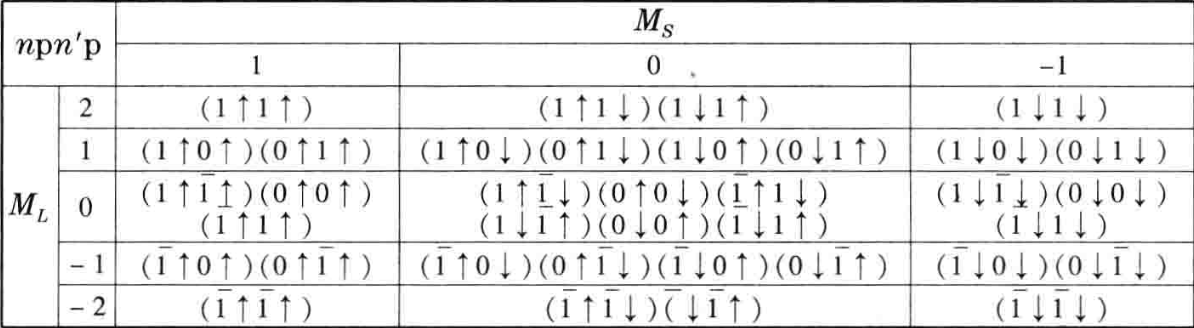
\includegraphics[scale=0.45]{fig/fig 5.4.png}
        \footnote{$\bar{1}=-1.$}
    \end{block}}
\only<2-3>{
    \begin{block}{$(n\mathrm{p})^2$}
        For equivalent electrons the Pauli exclusion principle restricts the states.
        \begin{center}
            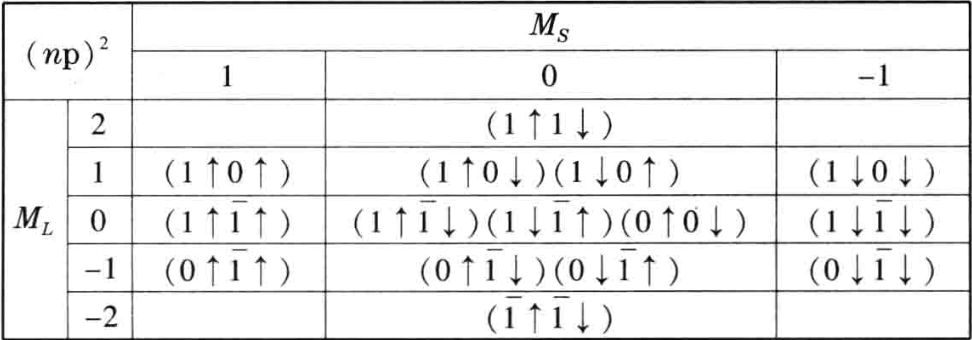
\includegraphics[scale=0.45]{fig/fig 5.5.png}
        \end{center}
        \begin{block}{Even rule:}<3>
            \begin{equation*}
                2|(L+S).
            \end{equation*}
        \end{block}
    \end{block}}
\only<4>{
    \begin{columns}
        \hspace*{1em}
        \column{0.47\textwidth}
            \begin{figure}
                \centering
                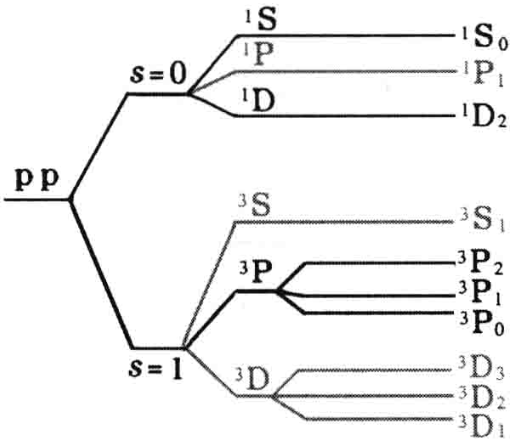
\includegraphics[scale=0.45]{fig/fig 5.6.png}
                \caption{pp electronic configuration energy levels}
            \end{figure}
        \column{0.54\textwidth}
            Black line: $(n\mathrm{p})^2$,\\
            Gray line: prohibited by Pauli's principle,\\
            All line: $n\mathrm{p}n'\mathrm{p}$.
    \end{columns}
}
\end{frame}

\begin{frame}{Hund's rules}
    \begin{block}{Hund's rules}
        \begin{enumerate}
            \item<1-> $S\nearrow\ E\searrow$;
            \item<2-> $L\nearrow\ E\searrow$;
            \item<3->
            \begin{itemize}
                \item<3-> Normal order ($J\searrow\ E\searrow$) : under half shell layer;
                \item<4-> Anomalous order ($J\nearrow\ E\searrow$) : over half shell layer.
            \end{itemize}
        \end{enumerate}
        \uncover<5->{However, Hund's rules are empirical and there are exceptions. They are more effective in inferring the ground state, with only a few exceptions. Using it to discuss excited states is not very reliable.}
    \end{block}
\uncover<6->{
    \begin{block}{Application: determine the ground state}
        \centering
        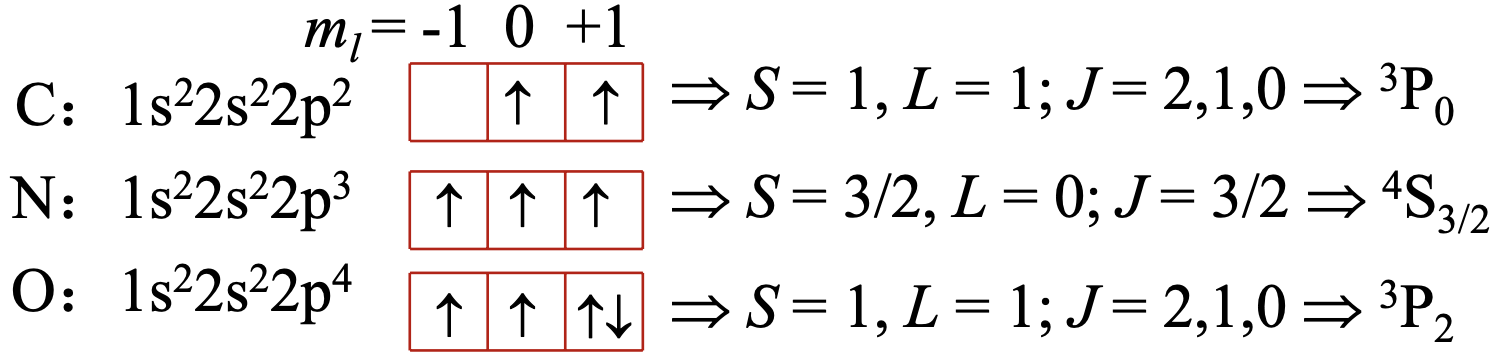
\includegraphics[scale=0.35]{fig/fig 5.7.png}
    \end{block}
    }
\end{frame}

\begin{frame}{Hund's rules}
    \begin{block}{Theoretical explanation}
    \uncover<1->{
        Generalize the potential expression of spin-orbit coupling to the coupling of any two angular momentum:
        \begin{equation*}
            U_{l_1l_2}=\frac1{2\mu^2c^2}\frac1r\frac{\mathrm{d}U}{\mathrm{d}r}{\boldsymbol{l}}_1\cdot{\boldsymbol{l}}_2,\quad (\boldsymbol{L}=\boldsymbol{l}_1+\boldsymbol{l}_2)
        \end{equation*}}
    \uncover<2->{
        The contribution of the coupling of angular momentum to the interaction potential: 
        \begin{equation*}
            \left\langle{\boldsymbol{l}}_1\cdot{\boldsymbol{l}}_2\right\rangle=\frac12\big[L(L+1)-l_1(l_1+1)-l_2(l_2+1)\big]\hbar^2.
        \end{equation*}}
    \uncover<3->{
        Apparently, $L\nearrow\ \left\langle{\boldsymbol{l}}_1\cdot{\boldsymbol{l}}_2\right\rangle\nearrow$, so the key is $\dfrac{\mathrm{d}U}{\mathrm{d}r}{~?~}0$.
        }
    \end{block}
\end{frame}

\begin{frame}{Hund's rules}
    \begin{block}{Theoretical explanation}
        \begin{itemize}
            \item<1-> Electron-electron Coulomb repulsion: 1\&2
            \begin{equation*}
                \frac{\mathrm{d}U}{\mathrm{d}r}\propto\frac{\mathrm{d}}{\mathrm{d}r}\left(\frac{e^2}{r}\right)\propto-\frac{1}{r^2}<0,
            \end{equation*}
            \item<2-> Electron-nucleon Coulomb attraction: 3-normal order
            \begin{equation*}
                \frac{\mathrm{d}U}{\mathrm{d}r}\propto\frac{\mathrm{d}}{\mathrm{d}r}\left(-\frac{e^2}{r}\right)\propto\frac{1}{r^2}>0,
            \end{equation*}
            \item<3-> Hole-nucleon Coulomb repulsion: 3-anomalous order
            \begin{equation*}
                \frac{\mathrm{d}U}{\mathrm{d}r}\propto\frac{\mathrm{d}}{\mathrm{d}r}\left(\frac{e^2}{r}\right)\propto-\frac{1}{r^2}<0.
            \end{equation*}
        \end{itemize}
    \end{block}
\end{frame}
\section{The jj-coupling scheme}

\begin{frame}{The jj-coupling scheme}
\uncover<1->{
    \begin{block}{Hamiltonian}
        $H_{\mathrm{s-o}}\gg H_{\mathrm{re}}$:
        \begin{equation*}
            \begin{aligned}
                H&=H_{\mathrm{CF}}+H_{\mathrm{s-o}}\\
                &=\sum_{i=1}^N\left\{-\frac{\hbar^2}{2m}\nabla_i^2+V_{\mathrm{CF}}\left(r_i\right)\right\}+\sum_{i=1}^N \xi_i(r_i)\boldsymbol{l}_1\cdot\boldsymbol{s}_i\\
                &=\sum_{i=1}^N\left\{-\frac{\hbar^2}{2m}\nabla_i^2+V_{\mathrm{CF}}\left(r_i\right)+ \xi_i(r_i)\boldsymbol{l}_1\cdot\boldsymbol{s}_i\right\}.
            \end{aligned}
        \end{equation*}
        \uncover<2->{
        Approximate to an independent particle system.}
    \end{block}}
\uncover<3->{
    Use a complete set of quantum numbers for each electron to characterize quantum states: eigenstates of $H_{\mathrm{s-o}}$: $\prod\limits_i^N\ket{n_i l_i j_i (m_j)_i}$.
    }
\end{frame}

\begin{frame}{The jj-coupling scheme}
\uncover<1->{
    Energy:
    \begin{equation*}
        \begin{aligned}
            E_{\mathrm{s-o}}&=\sum_{i}^{N} \expval{H_{\mathrm{s-o}}}{n_i l_i j_i (m_j)_i}\\
            &=\frac{1}{2}\sum_{i}^{N} \xi_{in_il_i}(r_i)[j_i(j_i+1)-l_i(l_i+1)-\frac{3}{4}].
        \end{aligned}
    \end{equation*}
    \begin{equation*}
        \hspace*{2.8em}(\xi_{in_il_i}(r_i)=\expval{\xi_i(r_i)}{n_il_i}.)
    \end{equation*}}
\uncover<2->{
    Therefore,
    \begin{equation*}
        \text{good quantum numbers}: j_1, j_2, \cdots, j_i, \cdots, j_N, J.
    \end{equation*}}
\uncover<3->{
    Label:
    \begin{equation*}
        (j_1, j_2, \cdots, j_i, \cdots, j_N)_J.
    \end{equation*}}
\uncover<4->{
    Considering $H_{\mathrm{re}}$, the energy levels will split according to the total angular momentum $\boldsymbol{J}$. (degeneracy with respect to $M_J$)
    }
\end{frame}

\begin{frame}{Example: pp electronic configuration}
\uncover<1->{
    \begin{block}{$n\mathrm{p}n'\mathrm{p}\ (n\neq n')$}
        \centering
        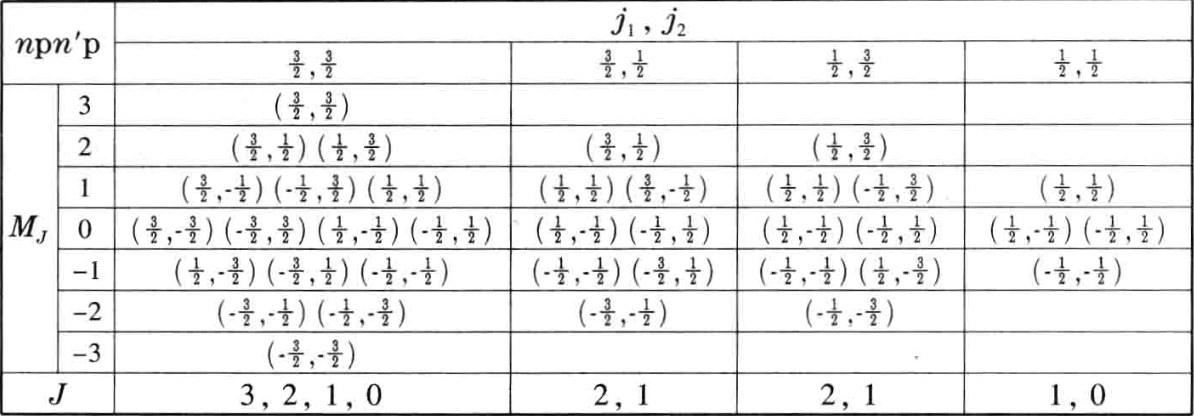
\includegraphics[scale=0.35]{fig/fig 5.8.png}
    \end{block}}
\uncover<2->{
    \begin{block}{$(n\mathrm{p})^2$}
        For equivalent electrons the Pauli exclusion principle restricts the states.
        \begin{center}
            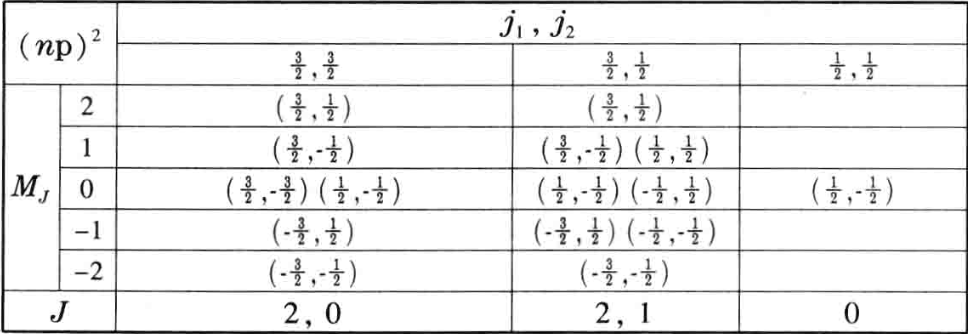
\includegraphics[scale=0.35]{fig/fig 5.9.png}
        \end{center}
    \end{block}}
\end{frame}
\section{Intermediate coupling: the transition between coupling schemes}

\begin{frame}{In theory}
    \begin{figure}
        \centering
        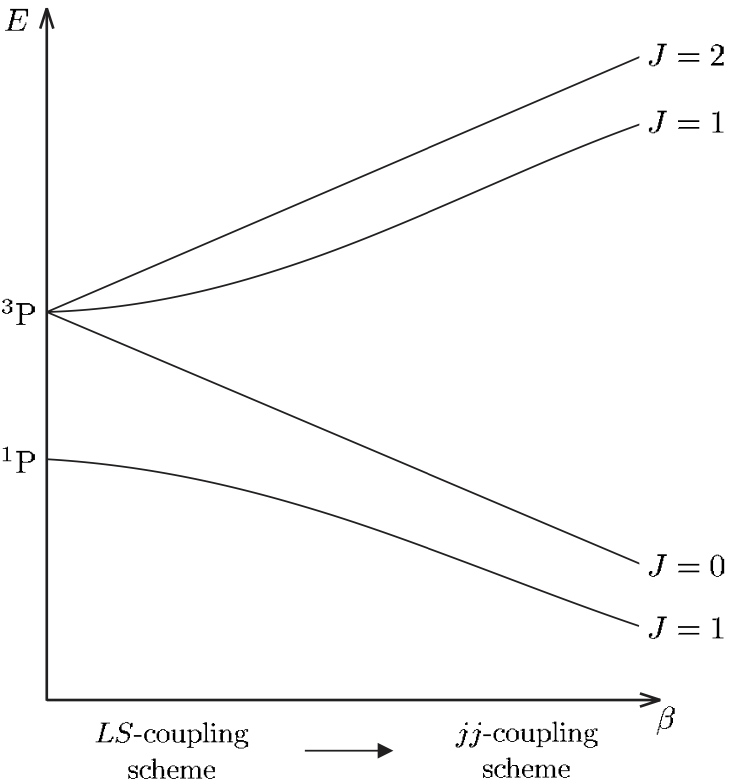
\includegraphics[scale=0.3]{fig/fig 5.10.png}
        \footnote{$\beta$: the spin–orbit interaction parameter.}
        \caption{sp configuration}
    \end{figure}
    
    As $\beta$ increases further the spin–orbit and residual electrostatic interactions become comparable and the LS-coupling scheme ceases to be a good approximation: the interval rule and (LS-coupling) selection rules break down. At large $\beta$ the jj-coupling scheme is appropriate.
\end{frame}

\begin{frame}{In theory and experiment}
    \begin{figure}
        \centering
        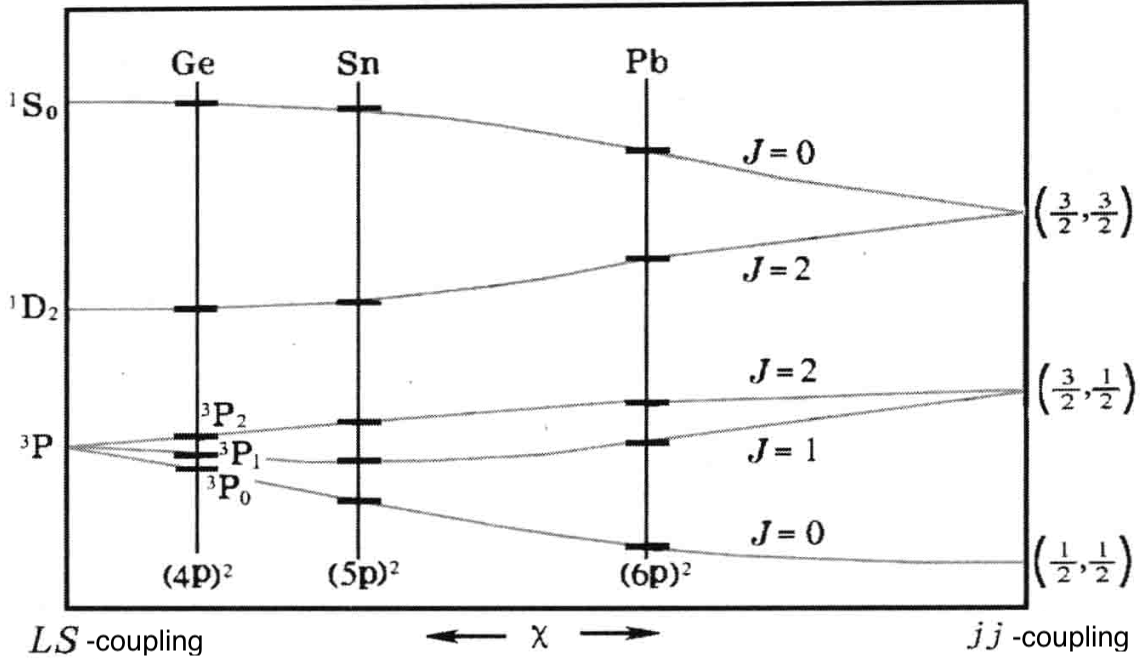
\includegraphics[scale=0.4]{fig/fig 5.11.png}
        \footnote{$\chi$: characteristic parameter.}
        \caption{$\mathrm{p}^2$ configuration}
    \end{figure}
    \centering
    A evident transition by $\chi$.
\end{frame}

\begin{frame}{In experiment}
    \begin{columns}
        \column{0.68\textwidth}
            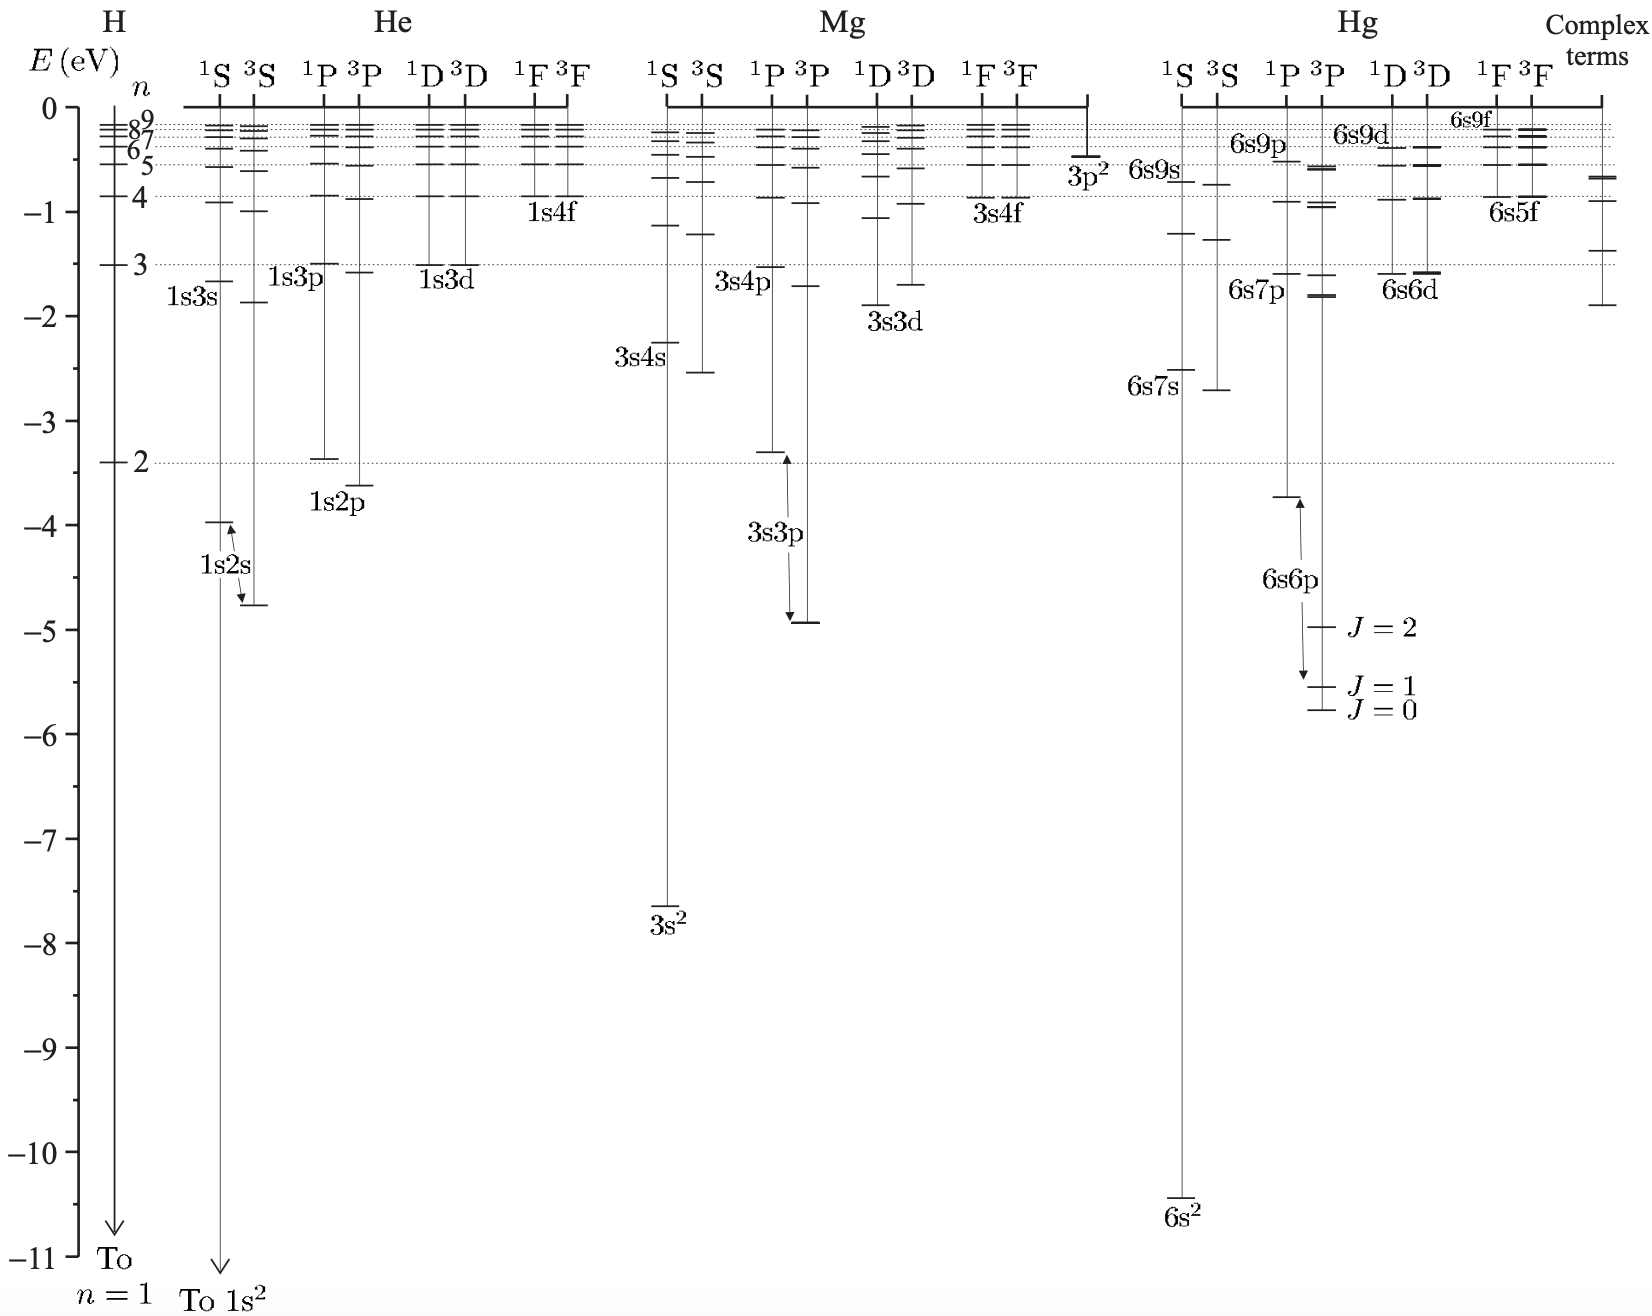
\includegraphics[scale=0.28]{fig/fig 5.12.png}
            Even for Hg, the LS-coupling scheme gives a closer approximation than the jj-coupling scheme.
    \only<2>{
        \column{0.36\textwidth}
            \begin{table}
                \centering
                \begin{tabular}{cc}
                    \hline
                    3s3p, Mg & 6s6p, Hg \\
                    \hline
                    2.1850 & 3.76 \\
                    2.1870 & 3.94 \\
                    2.1911 & 4.40 \\
                    3.5051 & 5.40 \\
                    \hline
                \end{tabular}
                \caption{$E$/\unit{m^{-1}}}
            \end{table}
            e.g. for the 6s6p configuration the $E_{\mathrm{re}}>E_{\mathrm{s-o}}$ but the interval rule is not obeyed because the spin-orbit interaction is not very small compared to the residual electrostatic interaction.}
    \only<3>{
        \column{0.36\textwidth}
            \begin{table}[]
                \centering
                \begin{tabular}{c|c}
                    \hline
                    $J$ & $E$ (\unit{m^{-1}}) \\
                    \hline
                    2 & 16908687 \\
                    1 & 16908694 \\
                    0 & 16908793 \\
                    1 & 17113500 \\
                    \hline
                \end{tabular}
                \caption{The 1s2p configuration in helium}
            \end{table}
            The interval rule is not obeyed: This occurs in helium because spin–spin and spin–other-orbit interactions have an energy comparable with that of the spin–orbit interaction.}
    \end{columns}
\end{frame}
\section{Selection rules in the LS-coupling scheme}

\begin{frame}{Electric dipole selection rules}
\only<1,5-6>{
    \begin{block}{Single electron}
        From conservation laws and quantum mechanics calculations:
        \begin{equation*}
            \begin{cases}
                    \Delta j=0, \pm1 \quad &(j=0 \nleftrightarrow j'=0),\\
                    \Delta m_j=0, \pm1, \quad &(m_j=0 \nleftrightarrow m_{j'}=0 \text{ if } \Delta j=0),\\
                    \Delta l=\pm1,&\\
                    \Delta m_l=0, \pm1.&
            \end{cases}
        \end{equation*}
    \end{block}}
\only<2-4>{
    \uncover<2-4>{
    LS-coupling scheme:
    \begin{equation*}
        \begin{cases}
            \Delta J=0,\pm1\quad &(J=0\nleftrightarrow J'=0), \\
            \Delta M_J=0,\pm1\quad &(M_J=0\nrightarrow M_{J'}=0\text{ if }\Delta J=0), \\
            \text{Parity changes}, \\
            \Delta l=\pm1\quad &\text{One electron jump}, \\
            \Delta L=0^{\footnotesize 1},\pm1\quad & (L=0\nleftrightarrow L'=0), \\
            \Delta S=0^{\footnotesize 2}.&
        \end{cases}
    \end{equation*}}
    \uncover<3-4>{
        1.$\Delta L=0$ is possible in principle, but more than one electron must be excited to a high-energy state.}\\
    \uncover<4>{
        2.Exception: In the mercury atom, however, transitions with $\Delta S=1$ occur, such as $6\text{s}^2\ {}^1\mathrm{S}_0- 6\text{s}6\text{p }^3\mathrm{P} _1$, that gives a so-called intercombination line with a wavelength of 254 nm.}}
\only<5-6>{
    \uncover<5->{
    jj-coupling scheme (two electrons) :
    \begin{equation*}
        \begin{cases}
            \Delta j_1=0,\quad\Delta j_2=0,\pm1,\quad\text{or}&\Delta j_1=0,\pm1,\quad\Delta j_2=0,\\
            \Delta J=0,\pm1\quad (J=0\nleftrightarrow J'=0),
        \end{cases}
    \end{equation*}}
    \uncover<6->{
    In fact, many elements fall between these two extreme situations, and the selection rules on both sides are not strictly followed.}}
\end{frame}

\begin{frame}{Magnetic dipole selection rules}
\uncover<1->{
    \begin{block}{}
        According to the multipole expansion of electromagnetic interactions, the magnetic dipole interaction can be described as the interaction between magnetic moment and vector radius, with the coefficient being the first-order spherical harmonic function. \\
        Therefore, the interaction can be expressed as
        \begin{equation*}
            {H}^{\prime}\propto\cos\theta Y_{10}(\theta,\phi)\propto Y_{00}(\theta,\phi).
        \end{equation*}
    \end{block}}
\uncover<2->{
    Therefore, apart from having the same selection rules as electric dipole transitions, there are also angular momentum selection rules: 
    \begin{equation*}
        \Delta l=0.
    \end{equation*}}
\uncover<3->{
    Directly generalized to multi-electron atoms:
    \begin{equation*}
        \Delta n=0,
        \begin{cases}
            \Delta L=0, \quad &\Delta S=0, \\
            \Delta J=0, \pm1, \quad &\Delta M_J=0, \pm1.
        \end{cases}
    \end{equation*}
    }
\end{frame}
\section{The Zeeman effect}

\begin{frame}{About concepts}
\uncover<1->{
    \begin{block}{Original concepts}
        A atomic spectral lines split in an external magnetic field:
        \begin{equation*}
            \begin{cases}
                    3: \text{The normal Zeeman effect}.\\
                    \text{the other}: \text{The anomalous Zeeman effect}.
            \end{cases}
        \end{equation*}
    \end{block}}
\uncover<2->{
    Modern:\\
    In a strong field: Paschen-Back effect.\\
    In a weak field:
    \begin{equation*}
        \begin{cases}
                3: \text{The normal Zeeman effect}.\\
                \text{the other}: \text{The anomalous Zeeman effect}.
            \end{cases}
    \end{equation*}
    }
\end{frame}

\subsection{The Paschen-Back effect}

\begin{frame}{The Paschen-Back effect}
\uncover<1->{
    For LS-coupling scheme, the atom's magnetic moment:
    \begin{equation*}
        \boldsymbol{\mu}=-\mu_{\mathrm{B}}\boldsymbol{L}-g_{s}\mu_{\mathrm{B}}\boldsymbol{S}.
    \end{equation*}}
\uncover<2->{
    The interaction of the atom with an external magnetic field is described by
    \begin{equation*}
        H_{{\mathrm{ZE}}}=-\boldsymbol{\mu}\cdot\boldsymbol{B}.
    \end{equation*}}
\uncover<3->{
    In a strong field: consider total magnetic moment along the z-direction
    \begin{equation*}
        \mu_z=\mu_{sz}+\mu_{lz}=-2\mu_\mathrm{B}m_s-\mu_\mathrm{B}m_l=-(2m_s+m_l)\mu_\mathrm{B}.
    \end{equation*}}
\uncover<4->{
    Energy: 
    \begin{equation*}
        E_{\mathrm{ZE}}=-\mu_\mathrm{z}B=(2m_s+m_l)\mu_\mathrm{B}.
    \end{equation*}}
\uncover<5->{
    \begin{block}{Selection rules}
        \begin{equation*}
            \begin{cases}
                \Delta m_s=0\\
                \Delta m_l=0,\pm1
            \end{cases}
        \end{equation*}
    \end{block}}
\end{frame}

\begin{frame}{Example}
    \begin{figure}
        \centering
        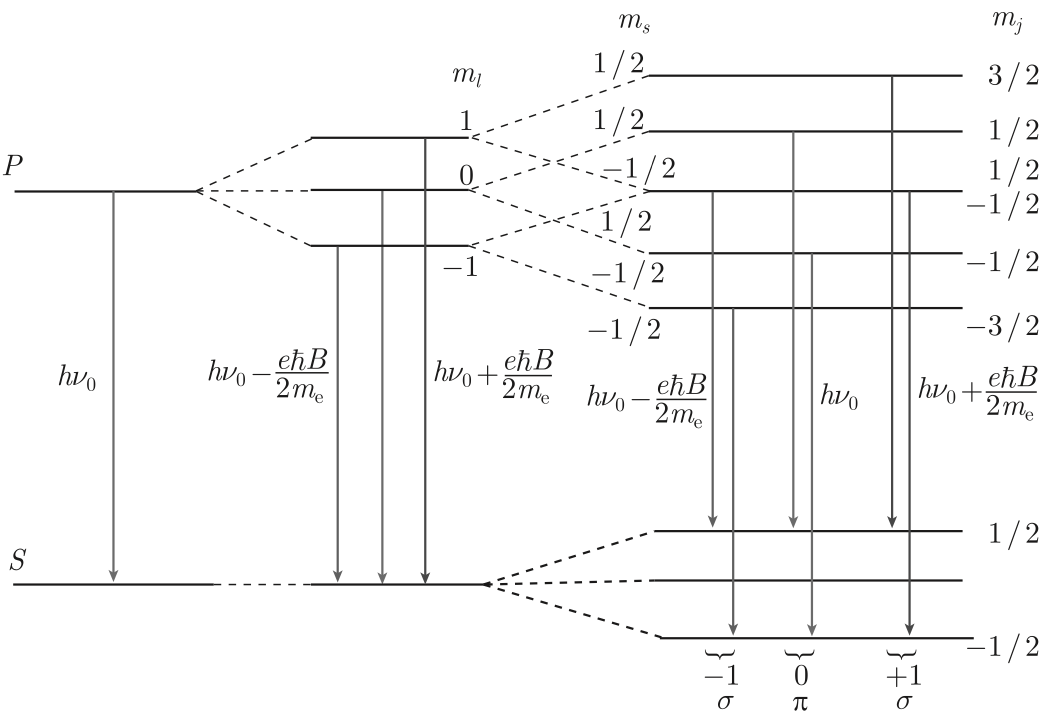
\includegraphics[scale=0.4]{fig/fig 5.13.png}
        \caption{$m_l=1, m_s=-\dfrac{1}{2},m_j=\dfrac{1}{2}$\&$m_l=-1,m_s=\dfrac{1}{2},m_j=-\dfrac{1}{2}$ are degenerate}
    \end{figure}
\end{frame}

\begin{frame}{The Zeeman effect}
\uncover<1->{
    In weak magnetic field, Hamiltonian: 
    \begin{equation*}
        H_{{\mathrm{ZE}}}=-\frac{\langle\boldsymbol{\mu}\cdot\boldsymbol{J}\rangle}{J\left(J+1\right)}\boldsymbol{J}\cdot\boldsymbol{B}=\frac{\langle\boldsymbol{L}\cdot\boldsymbol{J}\rangle+g_{s}\left\langle\boldsymbol{S}\cdot\boldsymbol{J}\right\rangle}{J\left(J+1\right)}\mu_{{\mathrm{B}}}BJ_{z}.
    \end{equation*}}
\uncover<2->{
    Energy: 
    \begin{equation*}
        E_{\mathrm{ZE}}=g_{J}\mu_{\mathrm{B}}BM_{J}.
    \end{equation*}}
\uncover<3->{
    Lande $g$-factor: 
    \begin{equation*}
        g_J=\frac{\langle\boldsymbol{L}\cdot\boldsymbol{J}\rangle+g_{s}\left\langle\boldsymbol{S}\cdot\boldsymbol{J}\right\rangle}{J\left(J+1\right)}.
    \end{equation*}
    }
\uncover<4->{
    Assuming that $g_s\simeq2$:
    \begin{equation*}
        g_J=\frac32+\frac{S\left(S+1\right)-L\left(L+1\right)}{2J\left(J+1\right)}.
    \end{equation*}
    }
\end{frame}

\begin{frame}{The Zeeman effect}
\uncover<1->{
    \begin{block}{No magnetic field}
        Consider $2\to1$:
        \begin{equation*}
            h\nu=E_2-E_1.
        \end{equation*}
    \end{block}}
\uncover<2->{
    External magnetic field $\boldsymbol{B}$:
    \begin{equation*}
        E_2'=E_2+g_2M_{J2}\mu_\text{B}B,\quad E_1'=E_1+g_1M_{J1}\mu_\text{B}B.
    \end{equation*}}
\uncover<3->{
    Spectral line splitting:
    \begin{equation*}
        E_2^{\prime}-E_1^{\prime}=h\nu+\left(g_2M_{J2}-g_1M_{J1}\right)\mu_\mathrm{B}B.
    \end{equation*}}
\uncover<4->{
    \begin{block}{Selection rules}
        \begin{equation*}
        \Delta M_J=0,\pm1.
    \end{equation*}
    \end{block}}
\end{frame}

\subsection{The normal Zeeman effect}

\begin{frame}{The normal Zeeman effect}
    \begin{figure}
        \centering
        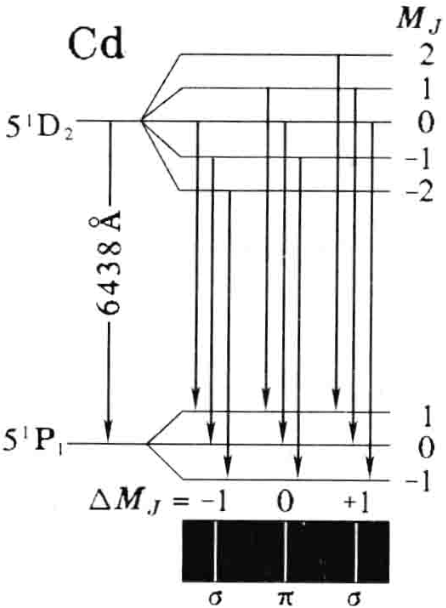
\includegraphics[scale=0.6]{fig/fig 5.14.png}
        \caption{Cd $5^1$D$_2\to5^1$P$_1:\,S_1=S_2=0\Rightarrow g_1=g_2=1$}
    \end{figure}
\end{frame}

\subsection{The anomalous Zeeman effect}

\begin{frame}{The anomalous Zeeman effect}
    \begin{figure}
        \centering
        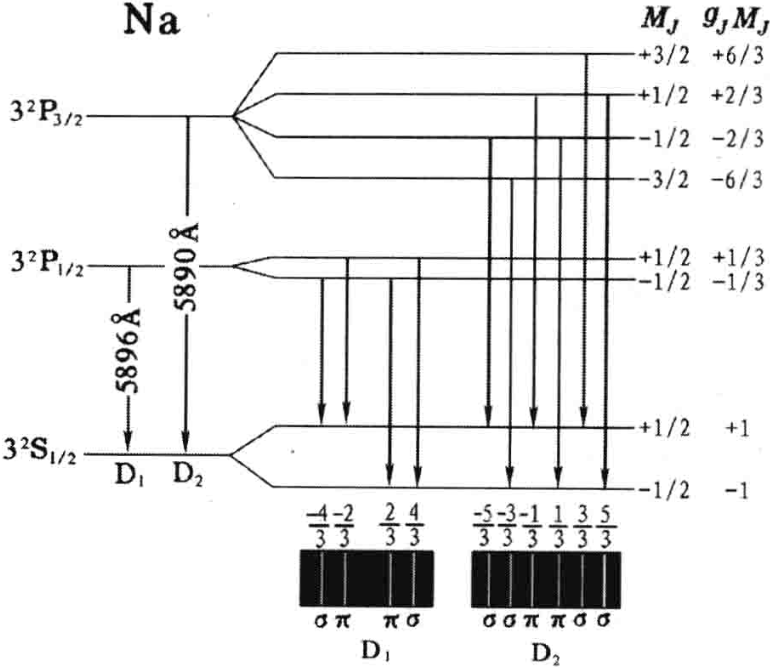
\includegraphics[scale=0.5]{fig/fig 5.15.png}
        \caption{Na $3^2$P$_{3/2}\to3^2$S$_{1/2}$/ $3^2$P$_{1/2}\to3^2$S$_{1/2}$}
    \end{figure}
\end{frame}
\section{Summary}

\begin{frame}{Summary}
\uncover<1->{
    \begin{figure}
        \centering
        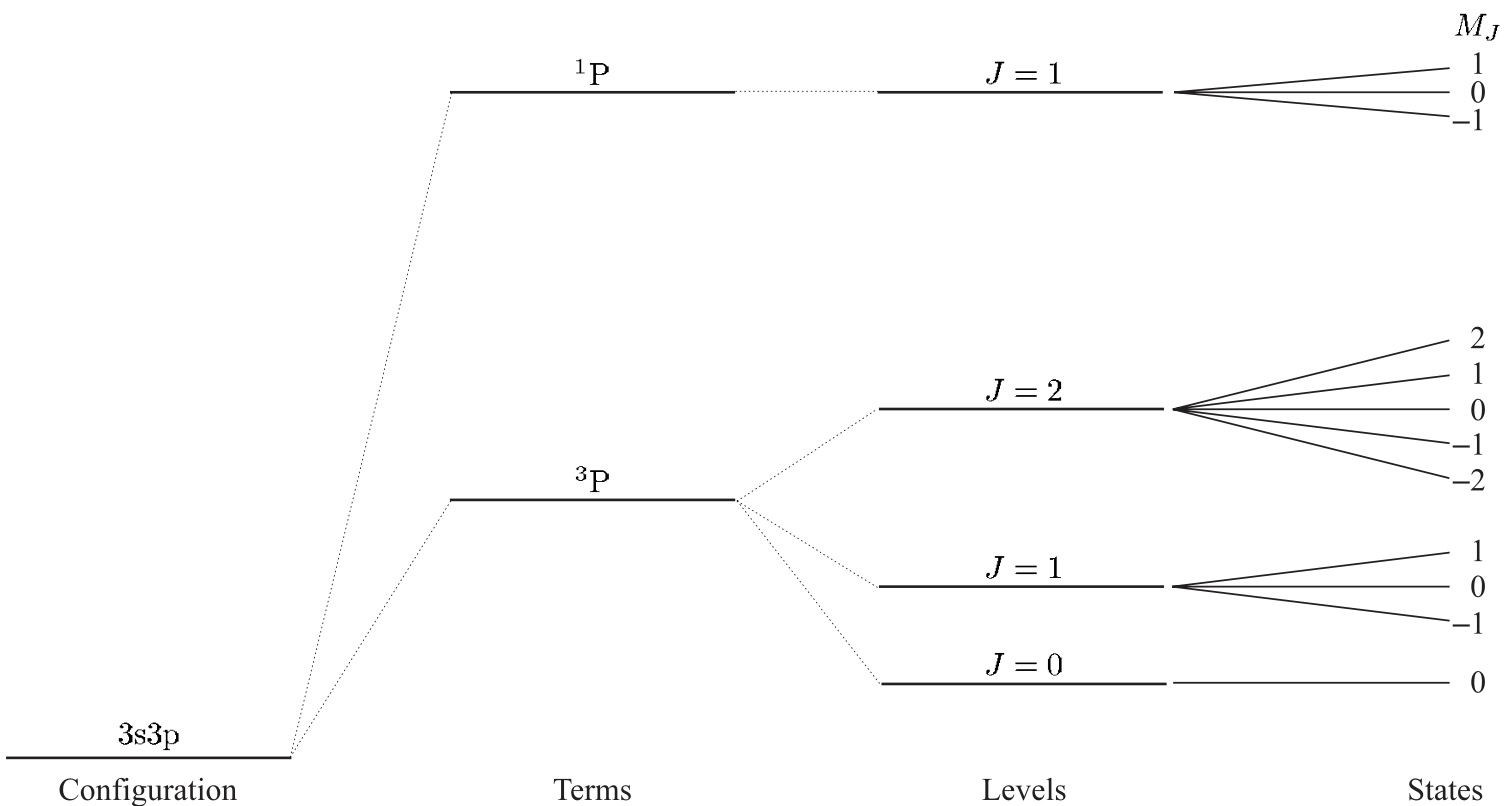
\includegraphics[scale=0.25]{fig/fig 5.16.png}
        \caption{The hierarchy of atomic structure for the 3s3p configuration of an alkaline earth metal atom.}
    \end{figure}}
\uncover<2->{
    Break down:\\
    (a) The residual electrostatic interaction is not small compared to the energy gap between the configurations.\\
    (b) The jj-coupling scheme is a better approximation than LS-coupling. \\
    (c) The Paschen–Back effect arises.}
\end{frame}

%reference,可惜只会用 IEEEtran。
\begin{frame}{Reference}
    \nocite{*}
    \bibliography{ref}
    \bibliographystyle{IEEEtran}
\end{frame}

%Q&A
\beamertemplateshadingbackground{structure.fg!90}{structure.fg}
\begin{frame}[plain]
	\vfill
	\centering
	{
		\centering \Huge \color{white}Q\&A
	}
	\vfill
\end{frame}

%Thank you
\beamertemplateshadingbackground{structure.fg!90}{structure.fg}
\begin{frame}[plain]
	\vfill
	\centering
	{
		\centering \Huge \color{white}Thank you for listening!
	}
	\vfill
\end{frame}

\end{document}